

\section{Limitations and Future Work}\looseness=-1
\label{section:discussion}

\begin{figure}[h]
	\centering
	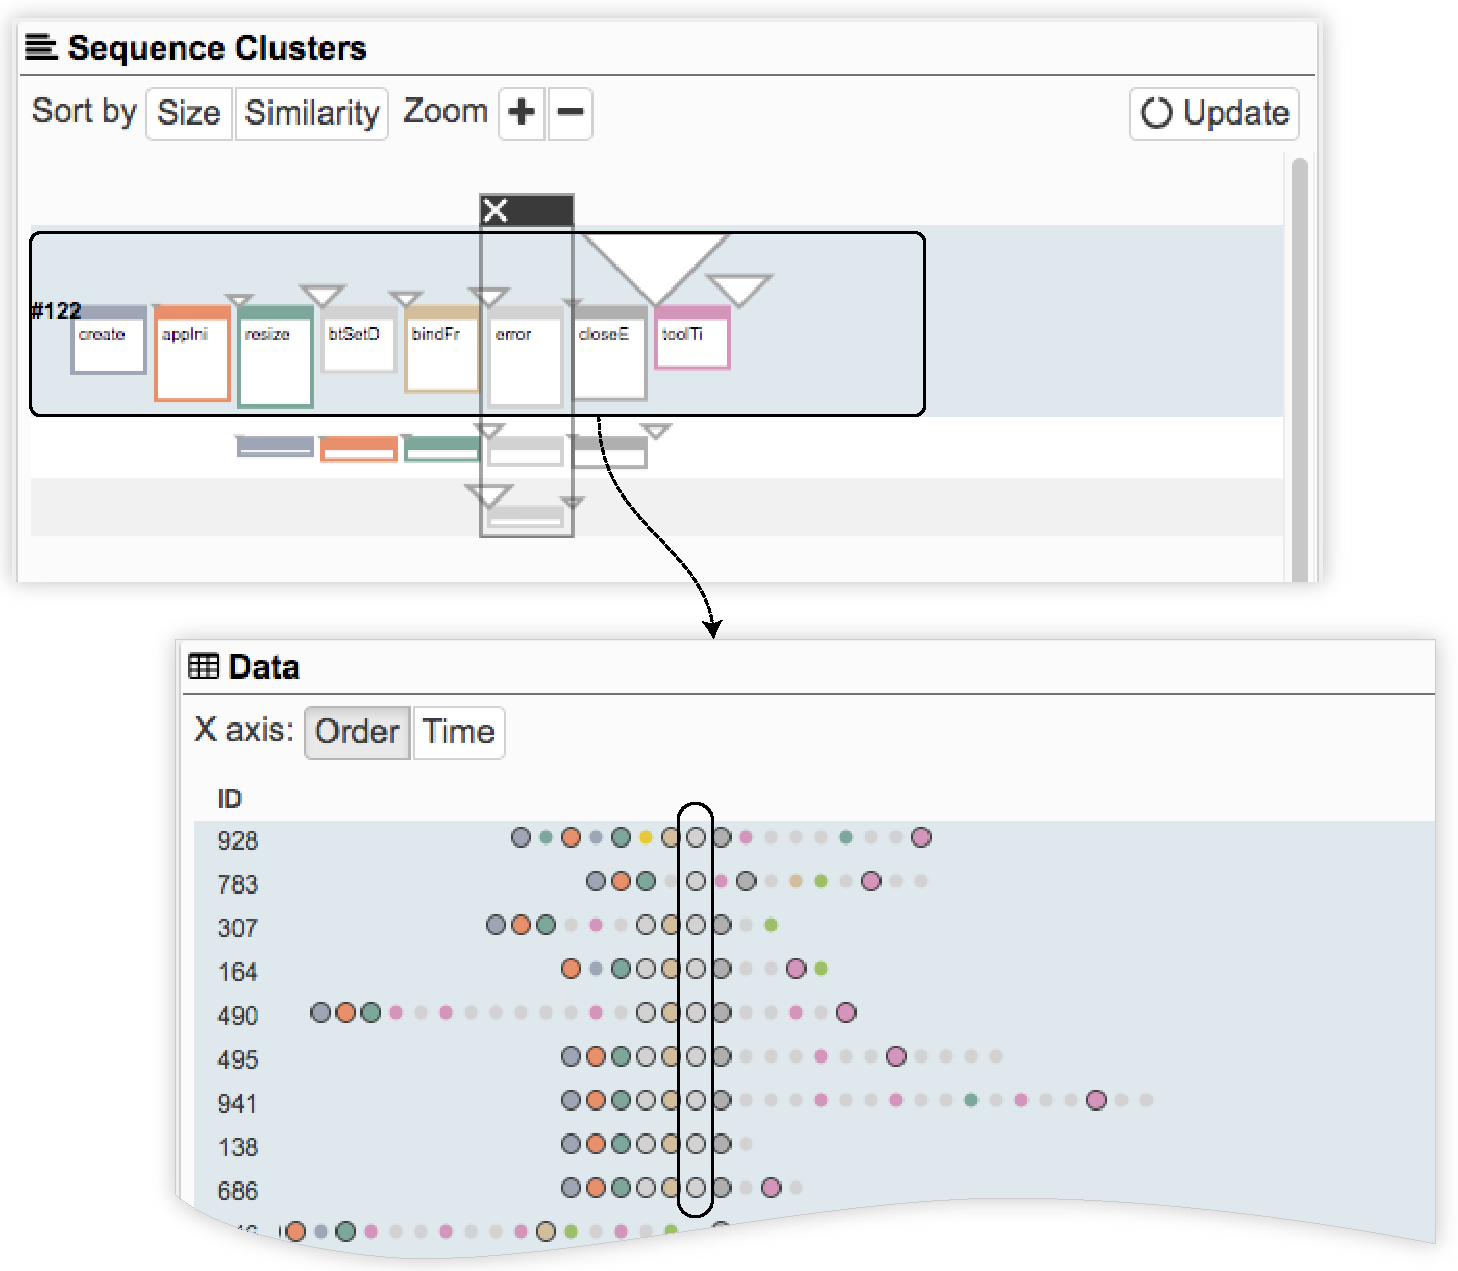
\includegraphics[width=0.9\linewidth]{pictures/case5}
	\caption{When aligned at the \textit{error} event, the summary view shows the most frequent antecedents (binding data) and sequelae (close error message window). 
		%		Insights derived from this can help the analysts identify potential flaws in the UI design.
	}
	\label{fig:case1_1}
\end{figure}

\revision{\textbf{Scalability.} The current visual design of the summary view can display 20$\sim$30 patterns without too much visual clutter. In the experiment, we tested a dataset containing up to about 2200 individual sequences and the result shows that dozens of patterns can effectively summarize the data. However some datasets may inherently contain more distinct patterns and the proposed approach could suffer from scalability issues. Further experiments need to be conducted to assess the applicability of the framework to large datasets. Besides that, one way to improve the scalability of the system is to extend the current framework to support hierarchical visual summary of event sequences. For example, starting from a high-level overview, users can select one cluster and split it into several low-level clusters. To support this extension, the algorithms need to maintain a hierarchical structure of the data, and the system features also need to be adjusted to support smooth user interaction. \looseness=-1}



\revision{\textbf{Multiple patterns.} The current framework only supports matching individual event sequences to a specific sequential pattern. In real-world applications, an event sequence may contain several patterns, especially when it is very long. We plan to tackle this issue from two directions. One direction is to extend the two-part representation and support matching individual sequences to multiple sequential patterns. Another direction is to design algorithms or support user interactions to segment long sequences into meaningful shorter ones and use the subsequences as input to the MDL framework.\looseness=-1}

\revision{\textbf{Event importance.} Although we treat all the events equally in the paper, it is common in real-world usage scenarios that some events are more critical compared to the others. For example, some faults in the vehicles may indicate failures in engine start and would require immediate repair services whereas others might not have major effect on vehicle operation. In such cases aggregating the critical events into the triangle may not be a good option. We will continue to explore the potential approaches to signify such differences in event importance.\looseness=-1}

\revision{\textbf{Pattern query.} In many usage scenarios, users are interested in certain sequences based on domain knowledge. To improve the usability of our system and keep users in the loop, the system should support pattern query and present the queried patterns in the summary view. \looseness=-1}



\revision{\textbf{General MDL based visual summary.} The method proposed in the paper addresses a fundamental trade-off in visualization design: reducing visual clutter vs. increasing the information content in the visualization. We believe our approach successfully showcases how this trade-off can be directly quantified and optimized to construct an informative and concise overview of the data. We \revision{envision} that similar approaches can also be designed for other types of data, e.g., graphs/networks and time series data. For example, Navlakha et. al. \cite{navlakha2008graph} has applied MDL for graph summarization. However, they did not address the tradeoff between the visual clutter and information content. For visualization community, there is still a lot of room for exploration.\looseness=-1}



